\documentclass{article}

%% PAQUETES

% Paquetes generales
\usepackage[margin=2cm, paperwidth=210mm, paperheight=297mm]{geometry}
\usepackage[spanish]{babel}
\usepackage[utf8]{inputenc}
\usepackage{gensymb}

% Paquetes para estilos
\usepackage{textcomp}
\usepackage{setspace}
\usepackage{colortbl}
\usepackage{color}
\usepackage{color}
\usepackage{upquote}
\usepackage{xcolor}
\usepackage{listings}
\usepackage{caption}
\usepackage[T1]{fontenc}
\usepackage[scaled]{beramono}

% Paquetes extras
\usepackage{amssymb}
\usepackage{float}
\usepackage{graphicx}
\usepackage{array}
\usepackage{multirow}
\usepackage{amsmath}
\usepackage{pifont} % Tick symbol

%% Fin PAQUETES


% Definición de preferencias para la impresión de código fuente.
%% Colores
\definecolor{gray99}{gray}{.99}
\definecolor{gray95}{gray}{.95}
\definecolor{gray75}{gray}{.75}
\definecolor{gray50}{gray}{.50}
\definecolor{keywords_blue}{rgb}{0.13,0.13,1}
\definecolor{comments_green}{rgb}{0,0.5,0}
\definecolor{strings_red}{rgb}{0.9,0,0}

%% Caja de código
\DeclareCaptionFont{white}{\color{white}}
\DeclareCaptionFont{style_labelfont}{\color{black}\textbf}
\DeclareCaptionFont{style_textfont}{\it\color{black}}
\DeclareCaptionFormat{listing}{\colorbox{gray95}{\parbox{16.78cm}{#1#2#3}}}
\captionsetup[lstlisting]{format=listing,labelfont=style_labelfont,textfont=style_textfont}

\lstset{
	aboveskip = {1.5\baselineskip},
	backgroundcolor = \color{gray99},
	basicstyle = \ttfamily\footnotesize,
	breakatwhitespace = true,   
	breaklines = true,
	captionpos = t,
	columns = fixed,
	commentstyle = \color{comments_green},
	escapeinside = {\%*}{*)}, 
	extendedchars = true,
	frame = lines,
	keywordstyle = \color{keywords_blue}\bfseries,
	language = Octave,                       
	numbers = left,
	numbersep = 5pt,
	numberstyle = \tiny\ttfamily\color{gray50},
	prebreak = \raisebox{0ex}[0ex][0ex]{\ensuremath{\hookleftarrow}},
	rulecolor = \color{gray75},
	showspaces = false,
	showstringspaces = false, 
	showtabs = false,
	stepnumber = 1,
	stringstyle = \color{strings_red},                                    
	tabsize = 2,
	title = \null, % Default value: title=\lstname
	upquote = true,                  
}

%% FIGURAS
\captionsetup[figure]{labelfont=bf,textfont=it}
%% TABLAS
\captionsetup[table]{labelfont=bf,textfont=it}


% COMANDOS

%% Titulo de las cajas de código
\renewcommand{\lstlistingname}{Código}
%% Titulo de las figuras
\renewcommand{\figurename}{Figura}
\addto\captionsspanish{\renewcommand{\figurename}{Figura}}
%% Titulo de las tablas
\renewcommand{\tablename}{Tabla}
\addto\captionsspanish{\renewcommand{\tablename}{Tabla}}
%% Referencia a los códigos
\newcommand{\refcode}[1]{\textit{Código \ref{#1}}}
%% Referencia a las imagenes
\newcommand{\refimage}[1]{\textit{Imagen \ref{#1}}}
%% Creación de símbolo tick
\newcommand{\tick}{\ding{52}}



\begin{document}


% OBJETIVOS
\section{Objetivos}

	El objetivo del trabajo práctico es la familiarización con el principio de funcionamiento del contador y sus controles. Además, se pretende que se conozca el correcto uso del instrumento para realizar mediciones de forma óptima. Por último, se espera poder identificar sus beneficios y limitaciones técnicas.
\bigskip\bigskip




% INTRODUCCIÓN
\section{Introducción Teórica}
	
	Un contador es un instrumento que cuenta la cantidad de pulsos o hemiciclos de la señal de entrada durante un intervalo de tiempo determinado manualmente o en función de una señal de referencia. Este instrumento puede usarse en diferentes configuraciones internas a fin de poder usarlo para hacer las siguientes mediciones:


\begin{itemize}
	\itemsep=3pt \topsep=0pt \partopsep=0pt \parskip=0pt \parsep=0pt
	
	\item Frecuencia
	\item Período
	\item Intervalo de tiempo
	\item Relación de frecuencias
\end{itemize}

	Dado que el contador es un instrumento digital, tiene la ventaja de no presentar errores de presentación y visualización que tienen los instrumentos analógicos, pero presenta otros tipos de errores inherentes a los instrumentos digitales.
\bigskip\bigskip



%% INTRODUCCIÓN - Medición de Frecuencia	
\subsection{Medición de Frecuencia}
\medskip

	En este modo, el contador cuenta durante el tiempo elegido en la \textit{Base de Tiempo}, la cantidad de ciclos de la señal de entrada. Ese valor es el que aparece en el display indicando la frecuencia.
\bigskip\bigskip


% Figura 1
\begin{figure}[h]
	\centering
	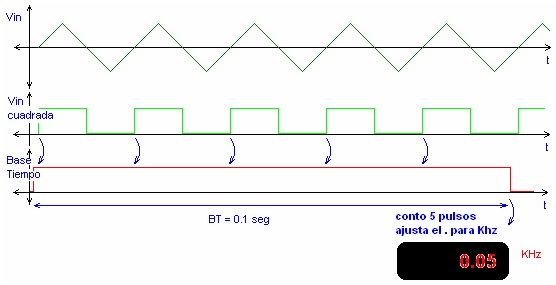
\includegraphics[width=0.63\textwidth]{images/01-ondasFrecuenciaContador.jpg}
	\medskip
	\caption{Esquema de conteo en la medición de frecuencia.}
\end{figure}
\bigskip\bigskip

	
	En la \textit{Figura 2} se muestra el diagrama en bloques basico del contador en este modo. El oscilador de la base de tiempos (BT) genera una señal de 10MHz, con una elevada estabilidad. Esta señal se aplica a un circuito divisor, de tal forma que a la salida se obtiene un pulso rectangular cuya duración es de 0.01, 0.1, 1 ó 10 segundos según sea seleccionado por el control \textit{GATE TIME}.A la señal de entrada , para eliminar ruidos que pueden causar una lectura errónea, se la transforma en una señal cuadrada. Para esto se la pasa por un disparador de Schmitt. Este disparador cuenta con un límite máximo de tensión y otro límite mínimo, y cuando la señal sobrepasa el máximo, o pasa por debajo del mínimo, la señal de salida (del disparador de Schmitt) varía. Un detalle importante es que los límites de tensión se pueden variar, por la razón de que puede darse el caso en el que la señal de entrada no supere los límites establecidos, de manera tal que no se llegue a formar una señal. Este pulso se aplica a la entrada IN-1 de la compuerta principal. El funcionamiento de la compuerta es tal que la señal de IN-2 se trasladará a la salida toda vez que IN-1 esté en estado alto. De este modo la entrada del contador de pulsos interno irá incrementando el número de cuentas acumuladas mientras la señal de gate este en estado alto. 
\bigskip


\newpage
% Figura 2
\begin{figure}[h]
	\centering
	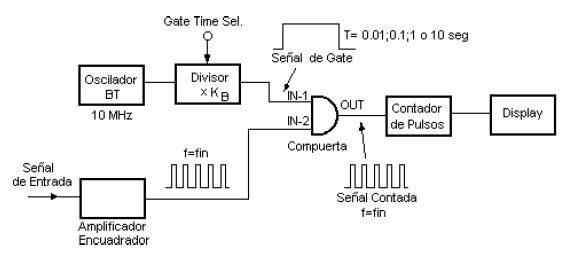
\includegraphics[width=0.75\textwidth]{images/02-diagrama-en-bloques-modo-medicion-frecuencia.jpg}
	\medskip
	\caption{Esquema de bloques de un contador convencional\\ en modo medición de frecuencias.}
\end{figure}
\bigskip\bigskip


	De esta manera, la frecuencia a medir será
\medskip

\begin{equation}
	f_x = {N_c \over T_G}
\end{equation}


\noindent donde, \\
$N_c$ = Número de cuentas acumuladas (ó ciclos de la señal de entrada);\\
$T_G$ = tiempo de apertura del Gate, comandado por la base de tiempos.
\bigskip\bigskip



%% INTRODUCCIÓN - Medición de Periodo	
\subsection {Medicion de Período}
\medskip

	En este modo, el contador cuenta la cantidad de pulsos de la base de tiempo durante un ciclo de la señal de entrada. A partir de ese valor obtiene el período. 
\bigskip\bigskip


% Figura 3
\begin{figure}[h]
	\centering
	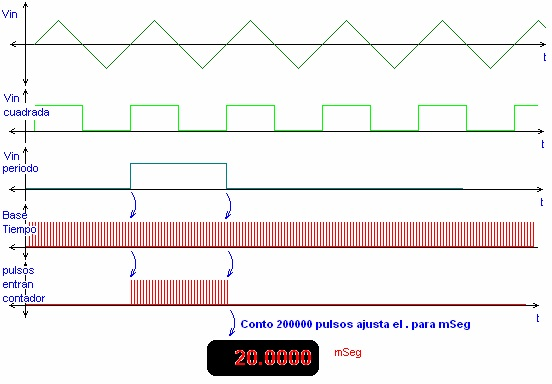
\includegraphics[width=0.70\textwidth]{images/03-ondasPeriodoContador.jpg}
	\medskip
	\caption{Esquema de conteo en la medición de período.}
\end{figure}
\bigskip\bigskip


	Más específicamente, en este modo de funcionamiento la señal contada es la de la base de datos (oscilador interno) mientras que el tiempo de apertura de la compuerta para conteo es fijado por la señal de entrada encuadrada y el acumulador de períodos como puede verse en el diagrama en bloques de la \textit{Figura 4}.
\bigskip\bigskip


% Figura 4
\begin{figure}[h]
	\centering
	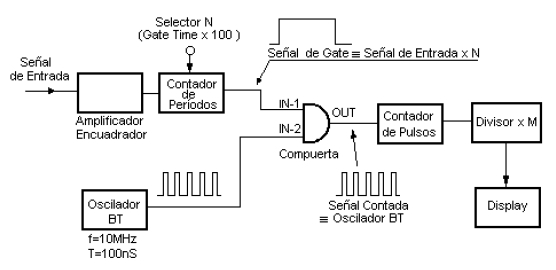
\includegraphics[width=0.75\textwidth]{images/04-diagrama-en-bloques-modo-medicion-periodo.jpg}
	\medskip
	\caption{Diagrama en bloques correspondiente al modo de\\ Medición de Período.}
\end{figure}
\bigskip\bigskip


	El contador de Períodos o acumulador cuenta la cantidad de eventos de la señal de entrada (N), y cierra la compuerta una vez alcanzada la cuenta prefijada por el control de Gate Time (1, 10, 100 ó 1000 períodos). Para un solo periodo medido (Gate Time = 0.01 segundo $\rightarrow$ N=1) resulta:
\medskip

\begin{equation}
	f_x = {N_c \over T_G}
\end{equation}
\medskip

\noindent donde $f_x = f_B = 1/t_B$, la frecuencia de la base de tiempos interna ($t_B$ el período de la misma) y $T_G = t_x$ el período de la señal de entrada que queremos medir, por lo que la ecuación (2) puede reescribirse para la medición en modo Período como:
\medskip

\begin{equation}
	t_x = {N_c \over f_B} = N_c \times t_B
\end{equation}
\bigskip\bigskip



%% INTRODUCCIÓN - Medición del Intervalo de tiempo	
\subsection{Medición del Intervalo de tiempo}
\medskip

	A diferencia de los tipos de mediciones expuestas en los apartados anteriores, en este caso el objetivo es medir el tiempo que transcurre entre dos eventos que pueden provenir de señales diferentes o de la misma señal.
	\par
	En este modo de funcionamiento ambos tipos de contadores, convencionales y recíprocos, lo hacen de la misma forma, ya que ambos acumulan y cuentan impulsos de la base de tiempos entre los eventos de apertura y cierre de la compuerta fijados a los canales 1 y 2. La expresión de cálculo del intervalo de tiempo es la misma que la del período (ecuación 7), donde el término $t_x$ deberá reemplazarse por $IT_x$ (intervalo de tiempo).
	\par
	En la \textit{Figura 5} se muestra el diagrama en bloques para este modo de medición. La salida del \textit{FLIP-FLOP} cambiará al estado alto cuando reciba una señal adecuada en la entrada SET. A partir de entonces ingnorará toda otra señal aplicada a SET hasta tanto no haya recibido una señal adecuada en la entrada RESET que lo vuelva al estado bajo.
	\par
	La pendiente de disparo de cada canal (flanco positivo o flanco negativo) puede variarse desde el panel frontal, permitiendo las diversas mediciones: ancho de pulso, período, fase, etc.
	\par
	A su vez, tanto los contadores convencionales como los recíprocos realizan mediciones de intervalos múltiples, cuya cantidad puede ser seleccionada desde el panel frontal (1, 10, 100 ó 1000 intervalos). La cuenta final se obtiene simplemente fijando el punto decimal de acuerdo a la cantidad de períodos seleccionados.
\bigskip\bigskip

\newpage
% Figura 5
\begin{figure}[h]
	\centering
	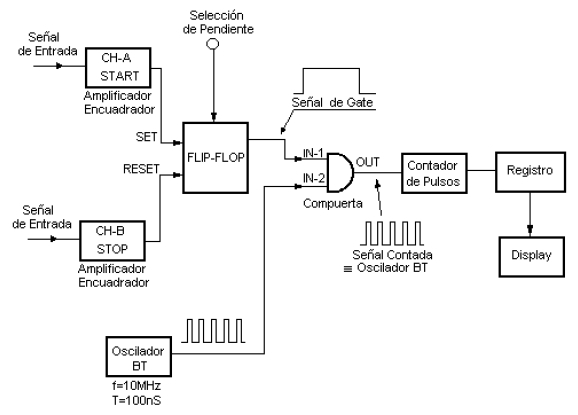
\includegraphics[width=0.75\textwidth]{images/05-diagrama-en-bloques-modo-intervalo-tiempos.jpg}
	\medskip
	\caption{Diagrama en bloques para la medición en modo\\ Intervalo de tiempos.}
\end{figure}
\bigskip\bigskip

	
	
%% INTRODUCCIÓN - Medición de la Relación de Frecuencias
\subsection{Medición de la Relación de Frecuencias} 
\medskip

	Esta última configuración permite comparar señales de frecuencias distintas, mostrando cuántos ciclos de una señal de alta frecuencia entran en un ciclo de la otra de frecuencia menor. Esto se logra utilizando la señal de menor frecuencia como Gate, conectada a un canal (habitualmente el B) y durante el tiempo de apertura de compuerta que determina esta, cuenta pulsos de la señal de mayor frecuencia, ingresada en el otro canal (habitualmente el A).
\bigskip\bigskip


% Figura 6
\begin{figure}[h]
	\centering
	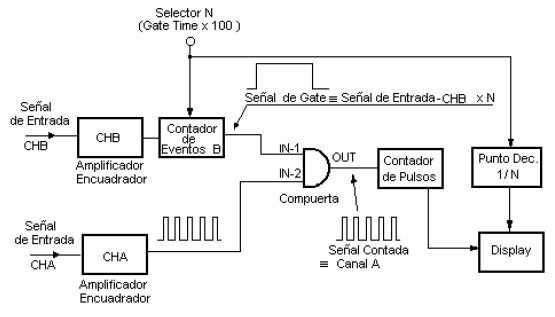
\includegraphics[width=0.75\textwidth]{images/06-diagrama-en-bloques-modo-relacion-frecuencias.jpg}
	\medskip
	\caption{Diagrama en bloques para la medición en modo\\ Intervalo de tiempos.}
\end{figure}
\bigskip\bigskip


	El diagrama en bloques correspondiente a este modo de funcionamiento se muestra en la \textit{Figura 6}. Para hacer una analogía podría asimilarse al modo medición de Período, donde el Período medido es de la señal B (menor frecuencia) y la Base de Tiempos es la señal A (mayor frecuencia). La lógica interna presentará luego en el display la cantidad de pulsos de A contados que es directamente la relación entre las frecuencias de los canales A y B. En el caso de realizar promediación de períodos, simplemente la lógica interna fija el punto decimal un lugar a la izquierda por cada década del multiplicador N (divide por N, que siempre son multiplos de 10, 1 - 10 - 100 ó 1000).
\bigskip\bigskip



%% INTRODUCCIÓN - Incertezas en las mediciones
\subsection{Incertezas en las mediciones} 
\medskip
	
	Como es de esperarse, las mediciones realizadas con el contador están afectadas por incertezas debido al propio funcionamiento del instrumento y varían según el tipo de medición que se esté llevando a cabo.
	\par
	Los errores que pueden aparecer son:

	\begin{itemize}
		\itemsep=3pt \topsep=0pt \partopsep=0pt \parskip=0pt \parsep=0pt
	
		\item Cuantización ó ``$\pm$1 cuenta''
		\item Disparo o trigger
		\item Base de tiempo
		\item Errores sistemáticos
	\end{itemize}
	\medskip

\noindent Para una amplia comprensión de cómo es que se obtienen las incertezas, diríjase al \textit{Apéndice A}.
\bigskip\bigskip




% MATERIALES UTILIZADOS
\section{Materiales utilizados}

	Se detalla a continuación (\textit{Tabla 1}) la lista de materiales y dispositivos utilizados durante el desarrollo de la práctica, acompañados por sus respectivas características y especificaciones principales. Para más información sobre el instrumental puede dirijirse a la sección \textit{Apéndice A}, ubicada al final del presente informe, donde se adjuntan las hojas de datos de todos estos.
\bigskip\bigskip


% Tabla 1
\begin{table}[!hbt]
	\begin{center}
	\begin{tabular}{|>{\centering\arraybackslash}m{5cm}|>{\arraybackslash}m{6cm}|}
		\hline
		\rowcolor[gray]{0.9}\textbf{Material/Instrumento} & \textbf{Especificaciones} \\
		\hline
		Generador de funciones & Modelo: 8140\\
		\hline
		Osciloscipio & \vbox{\hbox{\strut Marca: GOOD-WILL }
						   \hbox{\strut Modelo: 653G }}\\
		\hline
		Contador universal & \vbox{\hbox{\strut Marca: GOOD-WILL }
						   \hbox{\strut Modelo: GUC-2020 }}\\
		\hline
		Contador recíproco & \vbox{\hbox{\strut Marca: GOLDSTAR }
						   \hbox{\strut Modelo: FC-2130U / FC-2015U }}\\
		\hline
		Cables & Banana-Cocodrilo\newline Cocodrilo-Cocodrilo\newline BNC-BNC\newline Banana-BNC \\
		\hline
	\end{tabular}
	\caption{Listado de materiales e instrumental utilizado.}
	\end{center}
\end{table}
\bigskip\bigskip




% DESARROLLO
\section{Desarrollo}

	En los siguientes apartados se pasarán a desarrollar las mediciones empíricas, cada una de las cuales esta complementada con una explicación de los pasos llevados a cabo, valores obtenidos, análisis de resultados y conclusiones parciales.
\bigskip



%% DESARROLLO - Primer medición
\subsection{Primer medición}
\medskip
	
	En esta primer medición se dispondrán los contadores y el generador de la forma en que se muestra en la \textit{Figura 7}.
\bigskip

	
% Figura 7
\begin{figure}[h]
	\centering
	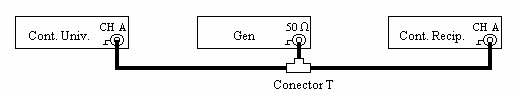
\includegraphics[width=0.70\textwidth]{images/07-bancoMedicion.jpg}
	\medskip
	\caption{Banco de medición para la primer medición.}
\end{figure}
\bigskip\bigskip


	Para el desarrollo de esta se generó una onda cuadrada de amplitud 5$V_{pp}$. Luego, se fue variando la frecuencia desde el generador de funciones, y se fue cambiando el modo y la base de tiempo de los contadores. De esta forma se obtuvieron los valores mostrados en la \textit{Tabla 2}.
\bigskip\bigskip


% Tabla 2
\begin{table}[!hbt]
	\begin{center}

		\begin{tabular}{|c|c|c|c|c|c|c|} \hline
			\multirow{2}{*}{\textbf{Frecuencia}}
			& \multicolumn{2}{c|}{\textbf{Contador recíproco}} & \multicolumn{2}{c|}{\textbf{Contador universal}} & \multirow{2}{*}{\textbf{Modo}} & \multirow{2}{*}{\textbf{Gate Time}} \\\cline{2-5}
			& Indicación display & Error(\%) & Indicación display & Error & & \\\hline
			
			\multirow{4}{*}{\textbf{10 Hz}}
			& 9,991893 Hz & 1e-5  & 0,010 KHz & 10 & Frecuencia & 1 Seg. \\\cline{2-7}
			& 100131,1 $\mu$S & 1e-5 & ¿OVER? &  & Período & 1 Seg. \\\cline{2-7}
			& - &  & ¿GATE? &  & Frecuencia & 0.01 Seg. \\\cline{2-7}
			& - &  & 100201,7 $\mu$S & 1e-5  & Período & 0.01 Seg. \\\hline

			\multirow{4}{*}{\textbf{1 kHz}}
			& 1,00423 kHz & 1e-4  & 1,005 kHz & 0,1  & Frecuencia & 1 Seg. \\\cline{2-7}
			& 995,7958 $\mu$S & 1e-5 & 995,797 $\mu$S & 1e-4 & Período & 1 Seg. \\\cline{2-7}
			& 1,0036 kHz & 0,01 & 1,0 kHz & 10 & Frecuencia & 0.01 Seg. \\\cline{2-7}
			& 996,43 $\mu$S & 1e-3 & 996,5 $\mu$S & 0,01 & Período & 0.01 Seg. \\\hline

			\multirow{4}{*}{\textbf{1 MHz}}
			& 1,001719 MHz & 1e-4 & 1001,743 kHz & 1e-4 & Frecuencia & 1 Seg. \\\cline{2-7}
			& 0,998182 $\mu$S & 1e-4 & 0,998 $\mu$S & 0,1 & Período & 1 Seg. \\\cline{2-7}
			& 1,0015 MHz & 1e-2 & 1001,5 kHz & 1e-2 & Frecuencia & 0.01 Seg. \\\cline{2-7}
			& 0,99868 $\mu$S & 1e-3 & 1,0 $\mu$S & 10 & Período & 0.01 Seg. \\\hline
		\end{tabular}

	\caption{Valores obtenidos en la primer medición.}
	\end{center}
\end{table}
\medskip\medskip


	En la \textit{Tabla 3} se muestran los valores calculados, correspondiente al análisis de las mediciones realizadas.
\bigskip\bigskip

% Tabla 3
\begin{table}[!hbt]
	\begin{center}

		\begin{tabular}{|c|c|c|c|c|c|c|} \hline
			\multirow{2}{*}{\textbf{Frecuencia}}
			& \multicolumn{3}{c|}{\textbf{Contador universal}} & \multicolumn{3}{c|}{\textbf{Contador recíproco}} \\\cline{2-7}
			& Modo (\textit{f} ó \textit{T}) & Gate time & Error & Modo (\textit{f} ó \textit{T}) & Gate time & Error \\\hline
			
			\textbf{10 Hz} & T & 0,01 & 1e-5 & Ambos & 1 & 1e-5 \\\hline
			\textbf{1 kHz} & T & 1 & 1e-4 & T & 1 & 1e-4 \\\hline
			\textbf{1 MHz} & f & 1 & 1e-4 & Ambos & 1 & 1e-4 \\\hline
		\end{tabular}

	\caption{Valores calculados para la primer medición.}
	\end{center}
\end{table}
\medskip\medskip

		
		De ambas tablas se desprende que el contador recíproco es mucho más preciso que el universal, por lo que su uso es útil en modo período o frecuencia cuando se mide frecuencias de cualquier magnitud. Por el contrario, en el unviersal, a fin de reducir los errores, se debe medir en modo frecuencia a frecuencias altas y en modo período a frecuencias bajas.


\newpage
%% DESARROLLO - Segunda medición
\subsection{Segunda medición}
\medskip

	En esta ocasión armaremos el banco de medición conectando el contador, el generador y el osciloscopio de la forma en la que se muestra en la \textit{Figura 8}.
\bigskip


% Figura 8
\begin{figure}[h]
	\centering
	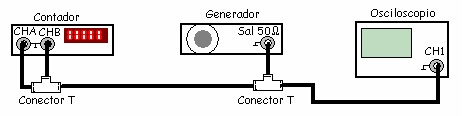
\includegraphics[width=0.63\textwidth]{images/08-bancoMedicionMed2.jpg}
	\medskip
	\caption{Banco de medición para la segunda medición.}
\end{figure}
\bigskip\bigskip	

	
	Para el desarrollo de esta medición se generó una onda cuadrada de amplitud 5V pico a pico, 1 KHz de frecuencia y se fue variando el ciclo de trabajo desde el generador y probando todas las combinaciones posibles entre el slope A y B ( + y -). 
	\par
	En la \textit{Tabla 4} se encuentran volcados los valores obtenidos en la realización de esta segunda experiencia.
\bigskip\bigskip\medskip


% Tabla 4
\begin{table}[!hbt]
	\begin{center}

		\begin{tabular}{|c|c|c|c|c|c|c|c|c|c|c|} \hline
			\multirow{3}{*}{\textbf{Duty Cycle}}
			& \multicolumn{2}{c|}{\textbf{Slope A +}} & \multicolumn{2}{c|}{\textbf{Slope A +}} & \multicolumn{2}{c|}{\textbf{Slope A -}} & \multicolumn{2}{c|}{\textbf{Slope A -}} & \multicolumn{2}{c|}{\textbf{Duty Cycle}} \\
			& \multicolumn{2}{c|}{\textbf{Slope B +}} & \multicolumn{2}{c|}{\textbf{Slope B -}} & \multicolumn{2}{c|}{\textbf{Slope B +}} & \multicolumn{2}{c|}{\textbf{Slope B -}} & \multicolumn{2}{c|}{(calculado)} \\\cline{2-11}
			& \textbf{Display} & \textbf{Error} & \textbf{Display} & \textbf{Error} & \textbf{Display} & \textbf{Error} & \textbf{Display} & \textbf{Error} & \textbf{Valor} & \textbf{Error} \\\hline
			
			\textbf{20\%} & 996,34 &  & 263,78 &  & 730,77 &  & 994,57 &  &  &  \\\hline
			\textbf{50\%} & 998,35 &  & 509,70 &  & 502,35 &  & 996,43 &  &  &  \\\hline
			\textbf{80\%} & 1001,70 &  & 785,50 &  & 216,06 &  & 1002,65 &  &  &  \\\hline
		\end{tabular}

	\caption{Valores obtenidos en la segunda medición.}
	\end{center}
\end{table}
\bigskip

	
	El contador toma el intervalo de tiempo entre la señal del \textit{CH A} y la del \textit{CH B}. Como en este caso es la misma señal la que entra a ambos canales, el contador no tiene el tiempo suficiente de notar la diferencia de fase si ambas pendientes son positivas o negativas, es por eso que se mide el período. En los demás casos, se puede apreciar que la suma de los valores cuando A y B son + y -, respectivamente, y cuando son - y +, da un valor cercano al período de la señal.
\bigskip\bigskip


%% DESARROLLO - Tercera medición
\subsection{Tercera medición}
\medskip

Haciendo uso de la señal de calibración del osciloscopio, con una frecuencia de aproximadamente $1 khz$ (su valor se encuentra en \textit{tabla 6}), ésta se conectó al \textit{CH B} y del generador con una frecuencia variable (conectado al \textit{CH A}), en este ítem del trabajo práctico se buscó evaluar el funcionamiento del modo relación de frecuencias del contador.
\bigskip


% Tabla 5
\begin{table}[!hbt]
	\begin{center}
		\begin{tabular}{|c|c|c|} \hline
			\textbf{Frecuencia del generador} & \textbf{Lectura del display} & \textbf{Error} \\\hline
			100 Hz & 0,1 &  \\\hline
			1 kHz & 11 &  \\\hline
			10 kHz & 10,4 &  \\\hline
			100 kHz & 102,4 &  \\\hline
		\end{tabular}

	\caption{Valores obtenidos en la tercera medición.}
	\end{center}
\end{table}
\medskip


	Ya que el contador utiliza la señal del \textit{CH B} como señal de \textit{Gate}, y de este modo cuenta los flancos de la señal del \textit{CH A} durante el período  de la señal de \textit{Gate}, es de entender que el error sea grosero cuando se presenta una señal en el \textit{CH A} con una frecuencia inferior a la del \textit{CH B}, como se puede apreciar en la \textit{Tabla 5}. Para los demás valores, el error se encuentra en un valor aceptable, donde se pueden considerar válidas las mediciones.
\bigskip


% Tabla 6
\begin{table}[!hbt]
	\begin{center}
		\begin{tabular}{|c|c|} \hline
			\multicolumn{2}{|c|}{\textbf{Frecuencia de la señal de calibración}} \\\cline{1-2}
			\textbf{Lectura del display} & \textbf{Error} \\\hline
			999,807 & \\\hline
		\end{tabular}

	\caption{Valores obtenidos en la tercera medición.}
	\end{center}
\end{table}
\medskip



%% DESARROLLO - Cuarta medición
\subsection{Cuarta medición}
\medskip

	En este caso se armó un circuito más complejo que los anteriores, incorporando una resistencia y un capacitor en una configuración de filtro pasa–bajos. Para que el efecto de carga aportado por los instrumentos involucrados en las mediciones sea despreciable, se utilizó un capacitor de 100 nF que es varios ordenes mayor a la capacidad equivalente del conjunto osciloscopio – punta. Con el mismo objetivo, se utilizó una resistencia de 1 KΩ.
	\par
	Se configuró el generador en una onda sinusoidal de 10 Vpp. Se utilizó al contador para medir  intervalos de tiempo y frecuencias, con el tiempo de compuerta fijo en 1 segundo.
	\par
	Al osciloscopio se lo utilizó en modo dual, para ver ambas señales simultáneamente, configurando el disparo en modo choppeado de manera tal de poder observar correctamente el desfasaje. Para calcular el desfasaje se utilizó la fórmula:
\medskip

\begin{equation}
	\phi = {Tdif * 360° \over T} = {Tdif * f * 360°}
\end{equation}
\bigskip


	En la \textit{Tabla 7} se muestran los valores obtenidos en la presente medición junto con los errores correspondientes a cada una de las indicaciones visualizadas en el display.
\bigskip


% Tabla 7
\begin{table}[!hbt]
	\begin{center}

		\begin{tabular}{|c|c|c|c|c|c|c|} \hline
			\textbf{Frecuencia} & \multicolumn{2}{c|}{\textbf{Frecuencia medida}} & \multicolumn{2}{c|}{\textbf{Intervalo de tiempo medido}} & \multicolumn{2}{c|}{\textbf{desfasaje calculado}} \\\cline{2-7}
			\textbf{del generador} & Indicación display & Error & Indicación display & Error & Resultado & Error propagado \\\hline
			
			320 Hz & 326,6041 Hz & 0,31\% & 2978,705 $\mu$S & 0.0012\% & 16,93° & 0,31\% \\\hline
			1600 Hz & 1,611072 kHz & 0,06\% & 557,9888 $\mu$S & 0.0014\% & 36,01° & 0,06\% \\\hline
			8 kHz & 7,996636 kHz & 0,01\% & 96,55358 $\mu$S & 0.0022\% & 81,93° & 0,02\% \\\hline

		\end{tabular}

	\caption{Valores obtenidos en la cuarta medición.}
	\end{center}
\end{table}
\medskip



%% DESARROLLO - Quinta medición
\subsection{Quinta medición}


% Tabla 8
\begin{table}[!hbt]
	\begin{center}

		\begin{tabular}{|c|c|c|c|>{\centering}p{1.65cm}|c|} \hline
			\textbf{Amplitud} & \multicolumn{2}{c|}{\textbf{Tensión AC}} & \textbf{Lectura del} & \multicolumn{2}{c|}{\textbf{La medición es válida}} \\\cline{2-3}\cline{5-6}
			\textbf{sugerida} & \textbf{Lectura} & \textbf{Error} & \textbf{contador} & \textbf{Sí} & \textbf{No} \\\hline
			
			\textbf{5V} & 3,548 &  & 1,0 & \tick &  \\\hline
			\textbf{1V} & 0,677 &  & 1,1 &  &  \\\hline
			\textbf{0,5V} & 0,347 &  & 1,1 &  &  \\\hline
			\textbf{0,25V} & 0,173 &  & 1,2 &  &  \\\hline
			\textbf{0,05V} & 0,027 &  & 1,0 &  &  \\\hline
			\textbf{0,04V} & 0,019 &  & 0 &  &  \\\hline

		\end{tabular}

	\caption{Valores obtenidos en la quinta medición.}
	\end{center}
\end{table}
\medskip




% CONCLUSIONES
\section{Conclusiones}

	
	Al analizar los datos obtenidos y los cálculos realizados, se puede concluir que el contador es un elemento muy versátil a la hora de realizar mediciones de períodos y frecuencias. También arroja valores correctos y con incertezas muy controladas en sus modos de intervalo de tiempo y relación de frecuencia. Es decir, tiene una incerteza considerablemente menor que la del osciloscopio para este tipo de mediciones ya que al leer la medición directamente en un display estamos eliminando los errores de apreciación que se producen cuando uno mide en un osciloscopio. Estas diferencias entre ambos instrumentos se pueden apreciar en la \textit{Tabla 9}.
\bigskip\bigskip


% Tabla 9
\begin{table}[!hbt]
	\begin{center}
		\begin{tabular}{|c|c|c|c|} \hline
			\textbf{Equipo de medición} & \textbf{Frecuencia / Período} & \textbf{Desfasaje} & \textbf{Ancho de pulso} \\\hline
			Osciloscopio &  &  &  \\\hline
			Contador &  &  &  \\\hline
		\end{tabular}

	\caption{Cuadro comparativo de los ordenes de magnitud\\ de los errores de los equipos.}
	\end{center}
\end{table}
\bigskip


	Un dato importante que se obtuvo, y que fue mencionado en apartados anteriores, fue el hecho de que en modo frecuencia trabaja satisfactoriamente con frecuencia altas. A su vez, ocurre algo similar en el modo período, ya que es conveniente que los tiempos a medir sean grandes. En caso de tener que realizar una medición de una baja frecuencia, conviene utilizar su recíproco, esto es, medir el período.
	\par
	Por último, se observó la influencia del error de cuantización y su relación con los tiempos de compuerta, los cuales pueden ser determinantes a la hora de realizar correctamente una medición.


	


\newpage \textit{}
\newpage



% APÉNDICE A
\newpage
\vspace*{4cm}
\begin{center}
	\textbf{\Huge{Apéndice A}} \\
	\bigskip\bigskip
	\Large{\textit{``Hojas de datos de instrumentos de medición''}}
\end{center}


\newpage \textit{}
\newpage

\end{document}
